\let\negmedspace\undefined
\let\negthickspace\undefined
\documentclass[journal]{IEEEtran}
\usepackage[a5paper, margin=10mm, onecolumn]{geometry}
%\usepackage{lmodern} % Ensure lmodern is loaded for pdflatex
\usepackage{tfrupee} % Include tfrupee package

\setlength{\headheight}{1cm} % Set the height of the header box
\setlength{\headsep}{0mm}     % Set the distance between the header box and the top of the text

\usepackage{gvv-book}
\usepackage{gvv}
\usepackage{cite}
\usepackage{amsmath,amssymb,amsfonts,amsthm}
\usepackage{algorithmic}
\usepackage{graphicx}
\usepackage{textcomp}
\usepackage{xcolor}
\usepackage{txfonts}
\usepackage{listings}
\usepackage{enumitem}
\usepackage{mathtools}
\usepackage{gensymb}
\usepackage{comment}
\usepackage[breaklinks=true]{hyperref}
\usepackage{tkz-euclide} 
\usepackage{listings}
% \usepackage{gvv}                                        
\def\inputGnumericTable{}                                 
\usepackage[latin1]{inputenc}                                
\usepackage{color}                                            
\usepackage{array}                                            
\usepackage{longtable}                                       
\usepackage{calc}                                             
\usepackage{multirow}                                         
\usepackage{hhline}                                           
\usepackage{ifthen}                                           
\usepackage{lscape}
\begin{document}

\bibliographystyle{IEEEtran}
\vspace{3cm}

\title{1.1.10.30}
\author{EE24BTECH11018 - Durgi Swaraj Sharma}

% \maketitle
% \newpage
% \bigskip
{\let\newpage\relax\maketitle}

\renewcommand{\thefigure}{\theenumi}
\renewcommand{\thetable}{\theenumi}
\setlength{\intextsep}{10pt} % Space between text and floats


\numberwithin{equation}{enumi}
\numberwithin{figure}{enumi}
\renewcommand{\thetable}{\theenumi}

 \textbf{Question}:\\
The direction cosines of the vector \brak{2\hat{i}+2\hat{j}-\hat{k}} are \rule{1cm}{0.2pt}. \\

\textbf{Solution: }\\
The unit vector in the direction of the given vector is \\
\begin{align}
	\vec{A} = \frac{1}{\sqrt{9}} \myvec{2 \\ 2 \\ -1} \label{eq1.1.10.30.1}
\end{align}
\begin{align}
	\vec{A} = \frac{1}{3} \myvec{2 \\ 2 \\ -1} \label{eq1.1.10.30.2}
\end{align}

\begin{figure}[h]
        \centering
       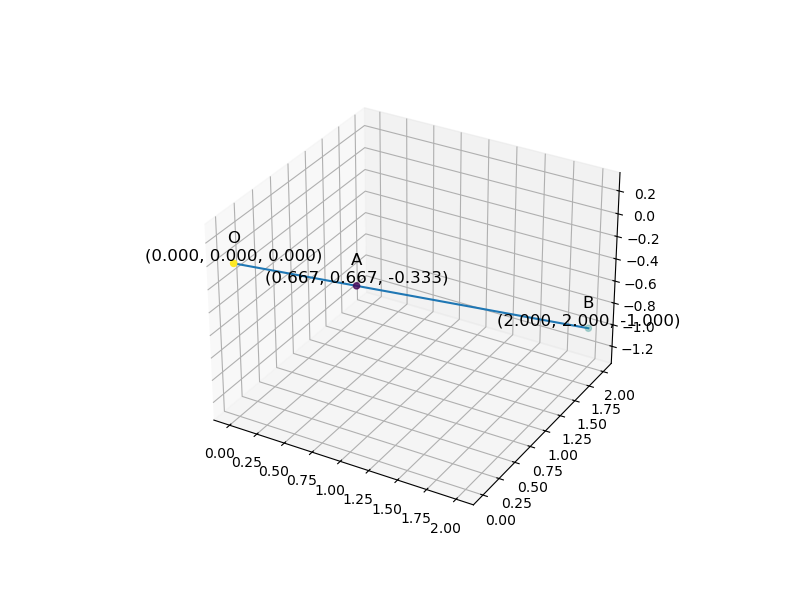
\includegraphics[width=0.7\linewidth]{/home/gvt1/Documents/sdcard/github/EE1030/Assignment4/figs/fig.png}  
       \caption{Vector B and Unit Vector A}
       \label{graph}
    \end{figure}

\end{document}
